%======================================================================
\chapter{Cross-Domain Relevance Transfer with BERT}
%======================================================================

\myworries{Need some images to fill it up...}

\section{Architecture}

\begin{figure}[b!]
\centering
  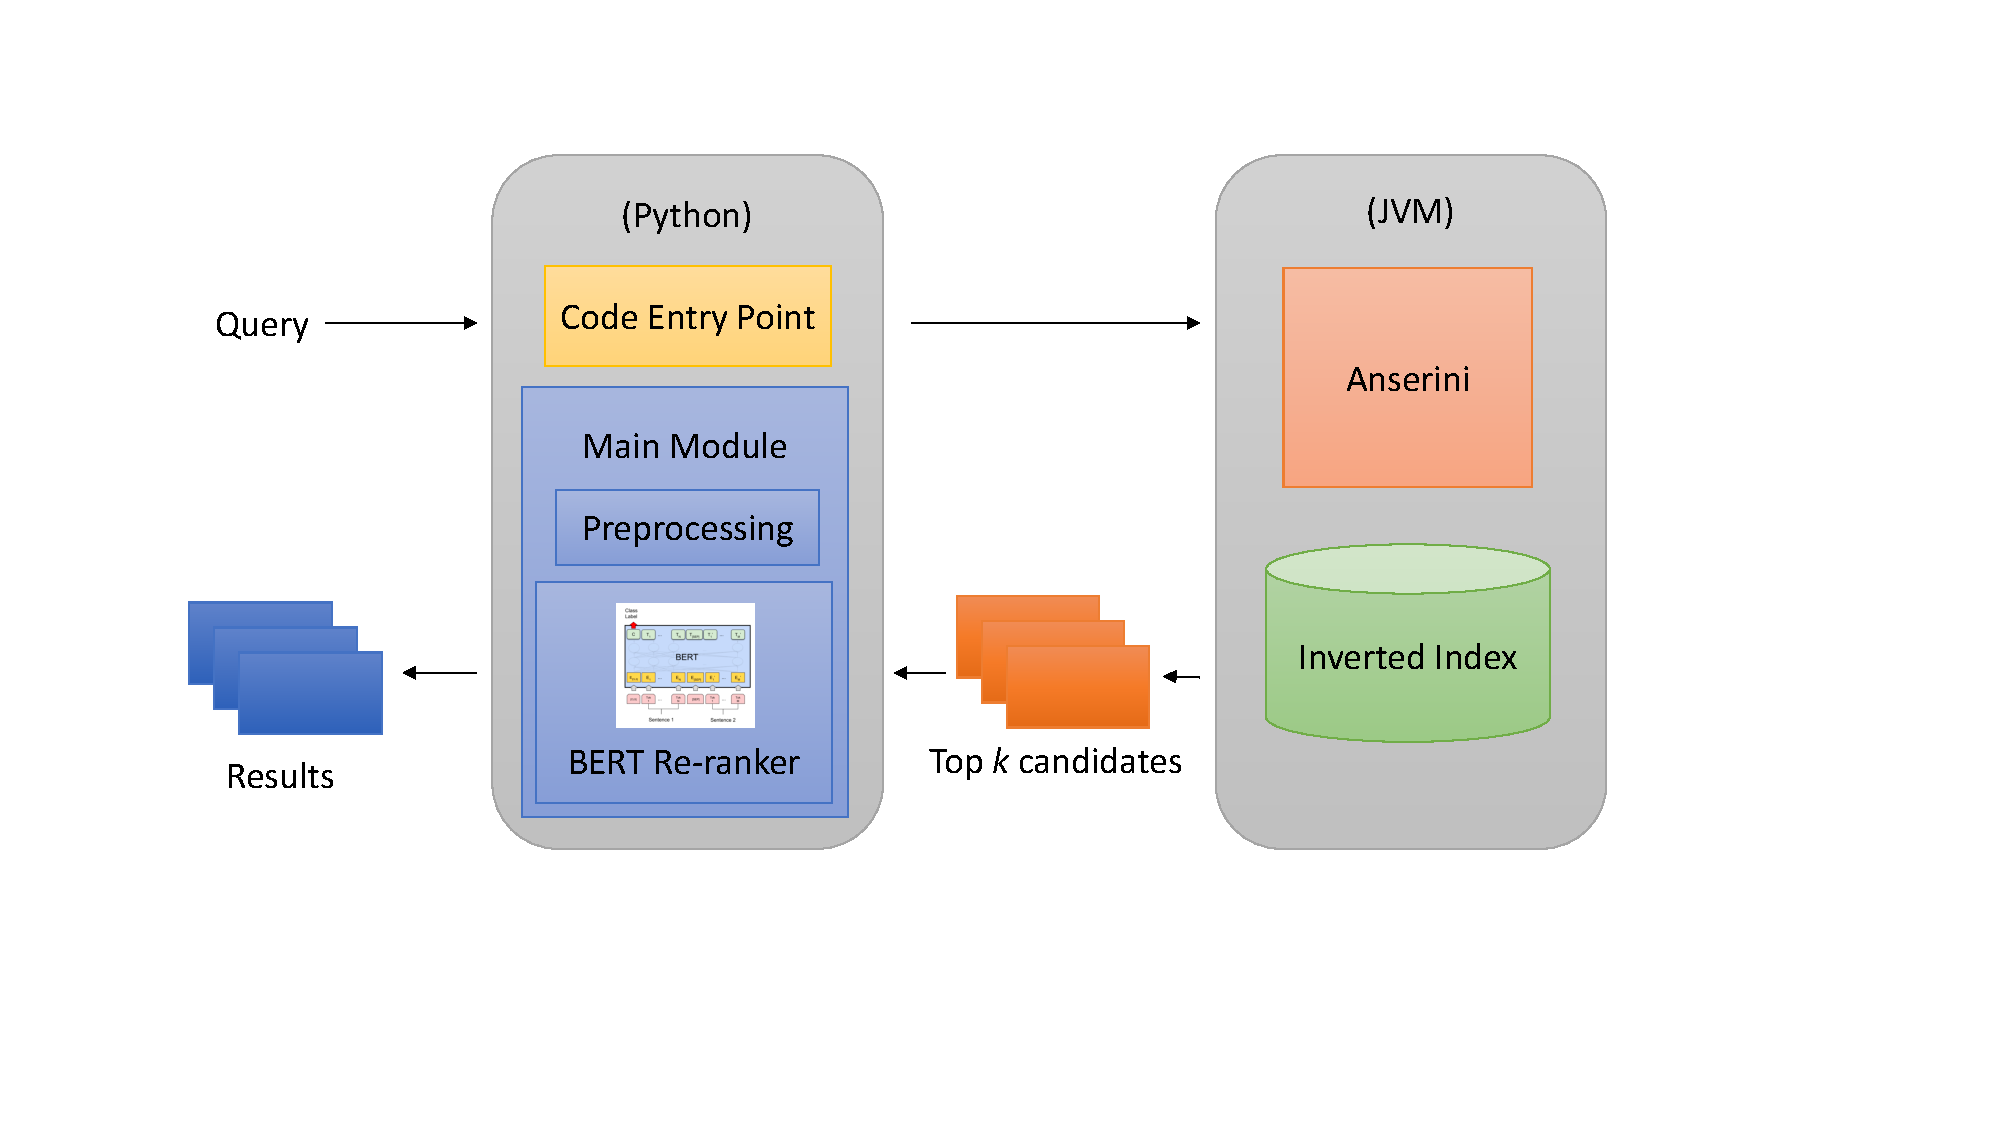
\includegraphics[width=5in]{architecture.pdf}
\caption{...}
\label{fig:arch}
\end{figure}

\myworries{General description? before or after?}
The architecture of our proposed system is shown in Figure \ref{fig:arch}, which is composed of a two-stage pipeline where Anserini is responsible for retrieval, the output of which is passed to a BERT-based reranker.
Our deep learning framework of choice is PyTorch \myworries{backend?} in Python.
\myworries{Nice transition...}

\subsection{Anserini}

\myworries{Anserini architecture, motivation...}

\myworries{Rationale for integration choices, demo stuff...}

\myworries{Reproducibility?}

\subsection{Integration}

\myworries{Smoother integration}
We apply BERT to document retrieval via integration with an open-source Anserini information retrieval toolkit.
Integration of NLP and IR capabilities with distinctly different \myworries{infrastructures} poses a number of technical challenges and requires certain design choices to be considered.
Applications of neural networks to document ranking usually involve multi-stage architectures, beginning with a traditional term-matching technique (e.g., BM25) over a standard inverted index, followed by a reranker that rescores the candidate list of documents~\cite{Asadi_Lin_SIGIR2013}.
\myworries{Anserini explanation here? Lucene indexes?}
Lucene is implemented in Java, and hence runs on the Java Virtual Machine (JVM).
However, most deep learning toolkits today, including TensorFlow and PyTorch, are written in Python with a C\texttt{++} backend.
Bridging Python and the JVM presents a technical challenge that needs to be address for an effective integration.

At the outset, we ruled out ``loosely-coupled'' integration approaches:
For example, passing intermediate text files is not a sustainable solution in the long term.
It is not only inefficient, but interchange formats frequently change (whether intentionally or accidentally), breaking code between multiple components.
We also ruled out integration via REST APIs for similar reasons:\ efficiency (overhead of HTTP calls) and stability (imperfect solutions for enforcing API contracts, particularly in a research environment).

There are a few options for the ``tightly-coupled'' integration we desired.
In principle, we could adopt the Java Virtual Machine (JVM) as the primary code entry point, with integration to the Torch backend via JNI, but this was ruled out because it would create two separate code paths (JVM to C\texttt{++} for execution and Python to C\texttt{++} for model development), which presents maintainability issues.
After some exploration, we decided on Python as the primary development environment, integrating Anserini using the Pyjnius Python library\footnote{\url{https://pyjnius.readthedocs.io/}} for accessing Java classes.
The library was originally developed to facilitate Android development in Python, and allows Python code to directly manipulate Java classes and objects.
Thus, Birch supports Python as the main development language (and code entry point, as shown in Figure~\ref{fig:arch}), connecting to the backend JVM to access retrieval capabilities.

\section{Model}

\myworries{How do we solve challenges? Innovations? Add a lot more here?}

\myworries{Go into details of BERT, then how we use it...}

\myworries{Maybe give example for how BERT for relevance modeling looks like? Input? May draw my own diagram}

\myworries{Can I add some math-y stuff to describe what BERT is doing?}

The core of our model is a BERT {\it sentence-level} relevance classifier.
\myworries{What does that mean?}
Following Nogueira et al.~\cite{nogueira2019passage}, this is framed as a binary classification task.
\myworries{Details!}

\subsection{Input Representation}

We form the input to BERT by concatenating the query $Q$ and a sentence $S$ into the sequence [\texttt{[CLS]}, $Q$, \texttt{[SEP]}, $S$, \texttt{[SEP]}] and padding each sequence in a mini-batch to the maximum length in the batch.
\myworries{What is Q and S for each dataset?}
We feed the final hidden state corresponding to the \texttt{[CLS]} token in the model to a single layer neural network whose output represents the probability that sentence $S$ is relevant to the query $Q$.
\myworries{Let's create a half page paragraph here}
\myworries{What is the BERT output? What does it mean?}
\myworries{Single layer neural network: MLP?}

\myworries{Motivation? Want to combine relevance matching signals}
To determine {\it document} relevance, we apply inference over each individual sentence in a candidate document, and then combine the top $ n $ scores with the original document score as follows:
\begin{equation} \label{eq:1}
S_f = a \cdot S_{doc}  + (1 - \alpha) \cdot \sum_{i = 1}^n w_i \cdot S_i
\end{equation}
\noindent where $ S_{doc} $ is the original document score and $ S_i $ is the $ i $-th top scoring sentence according to BERT.
In other words, the relevance score of a document comes from the combination of a document-level term-matching score and evidence contributions from the top sentences in the document as determined by the BERT model.
The parameters $ \alpha $ and the $ w_i $'s can be tuned via cross-validation.

\myworries{Go over everything to see if anything needs clarification...}

\section{Experimental Setup}

\subsection{Training and Inference with BERT}

We fine-tune $ \textrm{BERT}_{\textrm{\scriptsize Large}} $ \cite{devlin2018bert} on the datasets discussed in Section \ref{datasets}.
In our implementation we adopt the respective model's \texttt{BertForNextSentencePrediction} interface from the Huggingface \texttt{pytorch-transformers} (previously known as \texttt{pytorch-pretrained-bert}) library\footnote{https://github.com/huggingface/pytorch-transformers} as our base model.
The maximum sequence length, i.e: 512 tokens, is used for BERT in all our experiments.
We train all models using cross-entropy loss for 5 epochs with a batch size of 16.
We use Adam \cite{kingma2014adam} with an initial learning rate of $ 1 \times 10^{-5}$, linear learning rate warmup at a rate of 0.1 and decay of 0.1.
We conduct all our experiments on NVIDIA Tesla P40 GPUs with PyTorch v1.2.0.

\subsection{Evaluation}

\myworries{Elaborate?}
We retrieve an initial ranking of 1000 documents for each query in Robust04, Core17 and Core18 using the open-source Anserini information retrieval toolkit (\myworries{commit id}) based on Lucene 8.
To ensure fairness across all three collections, we use BM25 with RM3 query expansion with default parameters.
Before running inference with BERT to obtain relevance scores, we preprocess the retrieved documents.
First, we clean the documents by stripping any HTML/XML tags and split each document into its constituent sentences witih NLTK.
If the length of a sentence with the meta-tokens still exceeds the maximum input length of BERT, we further segment the spans into fixed sized chunks.
\myworries{CV?}

Based on preliminary exploration, we consider up to the top three sentences; any more does not appear to yield better results.
For Robust04, we follow the five-fold cross-validation settings in Lin et al.~\cite{lin2019neural} and Yang et al.~\cite{Yang_etal_SIGIR2019}; for Core17 and Core18 we similarly apply five-fold cross validation.
The parameters $\alpha$ and the $w_i$'s are learned via exhaustive grid search as follows:\ we fix $ w_1 = 1 $ and then vary $ a, w_2, w_3 \in [0, 1] $ with a step size 0.1, selecting the parameters that yield the highest average precision (AP).
Retrieval results are reported in terms of AP, precision at rank 20 (P@20), and NDCG@20.
We report retrieval effectiveness in terms of AP, P@20 and NDCG@20.